% Created by tikzDevice version 0.12 on 2019-01-16 14:48:27
% !TEX encoding = UTF-8 Unicode
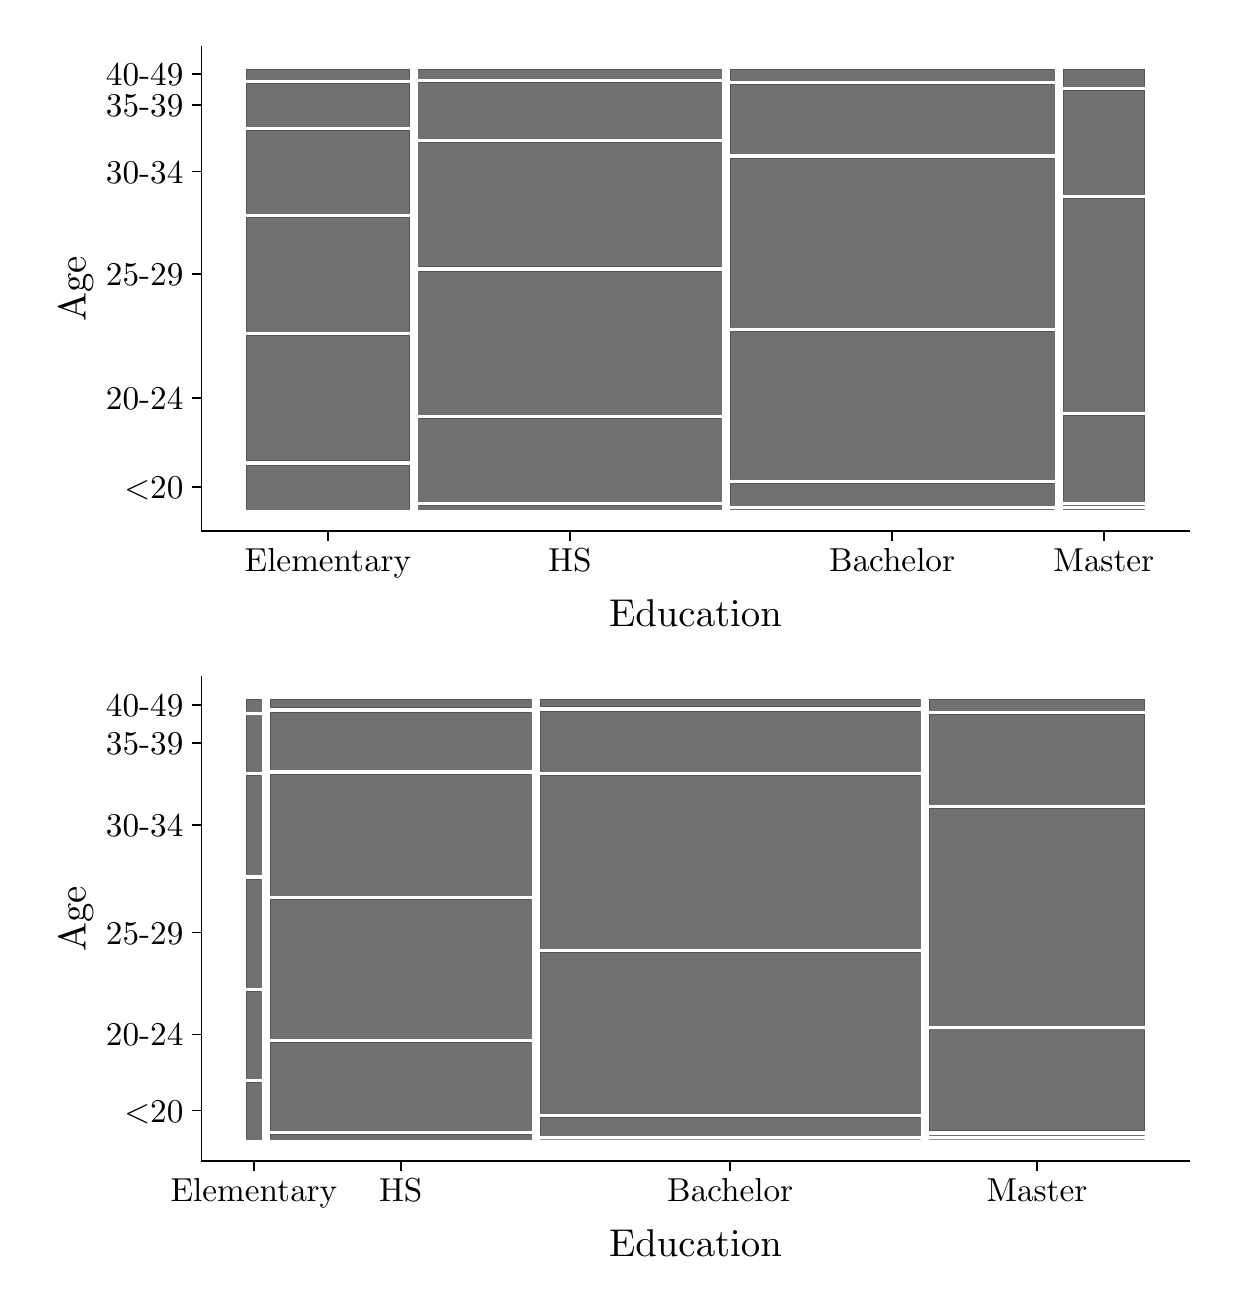
\begin{tikzpicture}[x=1pt,y=1pt]
\definecolor{fillColor}{RGB}{255,255,255}
\path[use as bounding box,fill=fillColor,fill opacity=0.00] (0,0) rectangle (426.79,455.24);
\begin{scope}
\path[clip] ( 62.78,273.33) rectangle (419.79,448.24);
\definecolor{drawColor}{RGB}{77,77,77}
\definecolor{fillColor}{RGB}{77,77,77}

\path[draw=drawColor,draw opacity=0.80,line width= 0.1pt,line join=round,fill=fillColor,fill opacity=0.80] ( 79.01,281.28) rectangle (138.02,297.28);

\path[draw=drawColor,draw opacity=0.80,line width= 0.1pt,line join=round,fill=fillColor,fill opacity=0.80] ( 79.01,298.80) rectangle (138.02,344.14);

\path[draw=drawColor,draw opacity=0.80,line width= 0.1pt,line join=round,fill=fillColor,fill opacity=0.80] ( 79.01,345.66) rectangle (138.02,386.76);

\path[draw=drawColor,draw opacity=0.80,line width= 0.1pt,line join=round,fill=fillColor,fill opacity=0.80] ( 79.01,388.28) rectangle (138.02,418.19);

\path[draw=drawColor,draw opacity=0.80,line width= 0.1pt,line join=round,fill=fillColor,fill opacity=0.80] ( 79.01,419.71) rectangle (138.02,435.09);

\path[draw=drawColor,draw opacity=0.80,line width= 0.1pt,line join=round,fill=fillColor,fill opacity=0.80] ( 79.01,436.60) rectangle (138.02,440.29);

\path[draw=drawColor,draw opacity=0.80,line width= 0.1pt,line join=round,fill=fillColor,fill opacity=0.80] (141.26,281.28) rectangle (250.54,282.64);

\path[draw=drawColor,draw opacity=0.80,line width= 0.1pt,line join=round,fill=fillColor,fill opacity=0.80] (141.26,284.15) rectangle (250.54,314.04);

\path[draw=drawColor,draw opacity=0.80,line width= 0.1pt,line join=round,fill=fillColor,fill opacity=0.80] (141.26,315.55) rectangle (250.54,367.38);

\path[draw=drawColor,draw opacity=0.80,line width= 0.1pt,line join=round,fill=fillColor,fill opacity=0.80] (141.26,368.90) rectangle (250.54,413.85);

\path[draw=drawColor,draw opacity=0.80,line width= 0.1pt,line join=round,fill=fillColor,fill opacity=0.80] (141.26,415.37) rectangle (250.54,435.46);

\path[draw=drawColor,draw opacity=0.80,line width= 0.1pt,line join=round,fill=fillColor,fill opacity=0.80] (141.26,436.98) rectangle (250.54,440.29);

\path[draw=drawColor,draw opacity=0.80,line width= 0.1pt,line join=round,fill=fillColor,fill opacity=0.80] (253.79,281.28) rectangle (370.94,281.28);

\path[draw=drawColor,draw opacity=0.80,line width= 0.1pt,line join=round,fill=fillColor,fill opacity=0.80] (253.79,282.79) rectangle (370.94,290.72);

\path[draw=drawColor,draw opacity=0.80,line width= 0.1pt,line join=round,fill=fillColor,fill opacity=0.80] (253.79,292.23) rectangle (370.94,345.68);

\path[draw=drawColor,draw opacity=0.80,line width= 0.1pt,line join=round,fill=fillColor,fill opacity=0.80] (253.79,347.20) rectangle (370.94,408.26);

\path[draw=drawColor,draw opacity=0.80,line width= 0.1pt,line join=round,fill=fillColor,fill opacity=0.80] (253.79,409.77) rectangle (370.94,434.88);

\path[draw=drawColor,draw opacity=0.80,line width= 0.1pt,line join=round,fill=fillColor,fill opacity=0.80] (253.79,436.40) rectangle (370.94,440.29);

\path[draw=drawColor,draw opacity=0.80,line width= 0.1pt,line join=round,fill=fillColor,fill opacity=0.80] (374.19,281.28) rectangle (403.56,281.28);

\path[draw=drawColor,draw opacity=0.80,line width= 0.1pt,line join=round,fill=fillColor,fill opacity=0.80] (374.19,282.79) rectangle (403.56,282.79);

\path[draw=drawColor,draw opacity=0.80,line width= 0.1pt,line join=round,fill=fillColor,fill opacity=0.80] (374.19,284.31) rectangle (403.56,315.26);

\path[draw=drawColor,draw opacity=0.80,line width= 0.1pt,line join=round,fill=fillColor,fill opacity=0.80] (374.19,316.78) rectangle (403.56,393.56);

\path[draw=drawColor,draw opacity=0.80,line width= 0.1pt,line join=round,fill=fillColor,fill opacity=0.80] (374.19,395.07) rectangle (403.56,432.71);

\path[draw=drawColor,draw opacity=0.80,line width= 0.1pt,line join=round,fill=fillColor,fill opacity=0.80] (374.19,434.23) rectangle (403.56,440.29);
\end{scope}
\begin{scope}
\path[clip] (  0.00,  0.00) rectangle (426.79,455.24);
\definecolor{drawColor}{RGB}{0,0,0}

\path[draw=drawColor,line width= 0.6pt,line join=round,line cap=rect] ( 62.78,273.33) --
	( 62.78,448.24);
\end{scope}
\begin{scope}
\path[clip] (  0.00,  0.00) rectangle (426.79,455.24);
\definecolor{drawColor}{RGB}{0,0,0}

\node[text=drawColor,anchor=base east,inner sep=0pt, outer sep=0pt, scale=  1.20] at ( 56.28,285.15) {\textless 20};

\node[text=drawColor,anchor=base east,inner sep=0pt, outer sep=0pt, scale=  1.20] at ( 56.28,317.34) {20-24};

\node[text=drawColor,anchor=base east,inner sep=0pt, outer sep=0pt, scale=  1.20] at ( 56.28,362.08) {25-29};

\node[text=drawColor,anchor=base east,inner sep=0pt, outer sep=0pt, scale=  1.20] at ( 56.28,399.10) {30-34};

\node[text=drawColor,anchor=base east,inner sep=0pt, outer sep=0pt, scale=  1.20] at ( 56.28,423.27) {35-39};

\node[text=drawColor,anchor=base east,inner sep=0pt, outer sep=0pt, scale=  1.20] at ( 56.28,434.32) {40-49};
\end{scope}
\begin{scope}
\path[clip] (  0.00,  0.00) rectangle (426.79,455.24);
\definecolor{drawColor}{RGB}{0,0,0}

\path[draw=drawColor,line width= 0.6pt,line join=round] ( 59.28,289.28) --
	( 62.78,289.28);

\path[draw=drawColor,line width= 0.6pt,line join=round] ( 59.28,321.47) --
	( 62.78,321.47);

\path[draw=drawColor,line width= 0.6pt,line join=round] ( 59.28,366.21) --
	( 62.78,366.21);

\path[draw=drawColor,line width= 0.6pt,line join=round] ( 59.28,403.23) --
	( 62.78,403.23);

\path[draw=drawColor,line width= 0.6pt,line join=round] ( 59.28,427.40) --
	( 62.78,427.40);

\path[draw=drawColor,line width= 0.6pt,line join=round] ( 59.28,438.45) --
	( 62.78,438.45);
\end{scope}
\begin{scope}
\path[clip] (  0.00,  0.00) rectangle (426.79,455.24);
\definecolor{drawColor}{RGB}{0,0,0}

\path[draw=drawColor,line width= 0.6pt,line join=round,line cap=rect] ( 62.78,273.33) --
	(419.79,273.33);
\end{scope}
\begin{scope}
\path[clip] (  0.00,  0.00) rectangle (426.79,455.24);
\definecolor{drawColor}{RGB}{0,0,0}

\path[draw=drawColor,line width= 0.6pt,line join=round] (108.51,269.83) --
	(108.51,273.33);

\path[draw=drawColor,line width= 0.6pt,line join=round] (195.90,269.83) --
	(195.90,273.33);

\path[draw=drawColor,line width= 0.6pt,line join=round] (312.36,269.83) --
	(312.36,273.33);

\path[draw=drawColor,line width= 0.6pt,line join=round] (388.87,269.83) --
	(388.87,273.33);
\end{scope}
\begin{scope}
\path[clip] (  0.00,  0.00) rectangle (426.79,455.24);
\definecolor{drawColor}{RGB}{0,0,0}

\node[text=drawColor,anchor=base,inner sep=0pt, outer sep=0pt, scale=  1.20] at (108.51,258.56) {Elementary};

\node[text=drawColor,anchor=base,inner sep=0pt, outer sep=0pt, scale=  1.20] at (195.90,258.56) {HS};

\node[text=drawColor,anchor=base,inner sep=0pt, outer sep=0pt, scale=  1.20] at (312.36,258.56) {Bachelor};

\node[text=drawColor,anchor=base,inner sep=0pt, outer sep=0pt, scale=  1.20] at (388.87,258.56) {Master};
\end{scope}
\begin{scope}
\path[clip] (  0.00,  0.00) rectangle (426.79,455.24);
\definecolor{drawColor}{RGB}{0,0,0}

\node[text=drawColor,anchor=base,inner sep=0pt, outer sep=0pt, scale=  1.40] at (241.29,238.95) {Education};
\end{scope}
\begin{scope}
\path[clip] (  0.00,  0.00) rectangle (426.79,455.24);
\definecolor{drawColor}{RGB}{0,0,0}

\node[text=drawColor,rotate= 90.00,anchor=base,inner sep=0pt, outer sep=0pt, scale=  1.40] at ( 20.97,360.79) {Age};
\end{scope}
\begin{scope}
\path[clip] ( 62.78, 45.70) rectangle (419.79,220.62);
\definecolor{drawColor}{RGB}{77,77,77}
\definecolor{fillColor}{RGB}{77,77,77}

\path[draw=drawColor,draw opacity=0.80,line width= 0.1pt,line join=round,fill=fillColor,fill opacity=0.80] ( 79.01, 53.66) rectangle ( 84.48, 74.14);

\path[draw=drawColor,draw opacity=0.80,line width= 0.1pt,line join=round,fill=fillColor,fill opacity=0.80] ( 79.01, 75.66) rectangle ( 84.48,107.18);

\path[draw=drawColor,draw opacity=0.80,line width= 0.1pt,line join=round,fill=fillColor,fill opacity=0.80] ( 79.01,108.70) rectangle ( 84.48,147.73);

\path[draw=drawColor,draw opacity=0.80,line width= 0.1pt,line join=round,fill=fillColor,fill opacity=0.80] ( 79.01,149.25) rectangle ( 84.48,185.23);

\path[draw=drawColor,draw opacity=0.80,line width= 0.1pt,line join=round,fill=fillColor,fill opacity=0.80] ( 79.01,186.75) rectangle ( 84.48,206.69);

\path[draw=drawColor,draw opacity=0.80,line width= 0.1pt,line join=round,fill=fillColor,fill opacity=0.80] ( 79.01,208.21) rectangle ( 84.48,212.67);

\path[draw=drawColor,draw opacity=0.80,line width= 0.1pt,line join=round,fill=fillColor,fill opacity=0.80] ( 87.72, 53.66) rectangle (181.87, 55.39);

\path[draw=drawColor,draw opacity=0.80,line width= 0.1pt,line join=round,fill=fillColor,fill opacity=0.80] ( 87.72, 56.91) rectangle (181.87, 88.54);

\path[draw=drawColor,draw opacity=0.80,line width= 0.1pt,line join=round,fill=fillColor,fill opacity=0.80] ( 87.72, 90.06) rectangle (181.87,140.25);

\path[draw=drawColor,draw opacity=0.80,line width= 0.1pt,line join=round,fill=fillColor,fill opacity=0.80] ( 87.72,141.76) rectangle (181.87,185.67);

\path[draw=drawColor,draw opacity=0.80,line width= 0.1pt,line join=round,fill=fillColor,fill opacity=0.80] ( 87.72,187.19) rectangle (181.87,208.05);

\path[draw=drawColor,draw opacity=0.80,line width= 0.1pt,line join=round,fill=fillColor,fill opacity=0.80] ( 87.72,209.57) rectangle (181.87,212.67);

\path[draw=drawColor,draw opacity=0.80,line width= 0.1pt,line join=round,fill=fillColor,fill opacity=0.80] (185.11, 53.66) rectangle (322.57, 53.66);

\path[draw=drawColor,draw opacity=0.80,line width= 0.1pt,line join=round,fill=fillColor,fill opacity=0.80] (185.11, 55.17) rectangle (322.57, 61.56);

\path[draw=drawColor,draw opacity=0.80,line width= 0.1pt,line join=round,fill=fillColor,fill opacity=0.80] (185.11, 63.07) rectangle (322.57,121.16);

\path[draw=drawColor,draw opacity=0.80,line width= 0.1pt,line join=round,fill=fillColor,fill opacity=0.80] (185.11,122.68) rectangle (322.57,185.24);

\path[draw=drawColor,draw opacity=0.80,line width= 0.1pt,line join=round,fill=fillColor,fill opacity=0.80] (185.11,186.75) rectangle (322.57,208.41);

\path[draw=drawColor,draw opacity=0.80,line width= 0.1pt,line join=round,fill=fillColor,fill opacity=0.80] (185.11,209.93) rectangle (322.57,212.67);

\path[draw=drawColor,draw opacity=0.80,line width= 0.1pt,line join=round,fill=fillColor,fill opacity=0.80] (325.82, 53.66) rectangle (403.56, 53.66);

\path[draw=drawColor,draw opacity=0.80,line width= 0.1pt,line join=round,fill=fillColor,fill opacity=0.80] (325.82, 55.17) rectangle (403.56, 55.17);

\path[draw=drawColor,draw opacity=0.80,line width= 0.1pt,line join=round,fill=fillColor,fill opacity=0.80] (325.82, 56.69) rectangle (403.56, 93.18);

\path[draw=drawColor,draw opacity=0.80,line width= 0.1pt,line join=round,fill=fillColor,fill opacity=0.80] (325.82, 94.70) rectangle (403.56,173.13);

\path[draw=drawColor,draw opacity=0.80,line width= 0.1pt,line join=round,fill=fillColor,fill opacity=0.80] (325.82,174.64) rectangle (403.56,207.19);

\path[draw=drawColor,draw opacity=0.80,line width= 0.1pt,line join=round,fill=fillColor,fill opacity=0.80] (325.82,208.70) rectangle (403.56,212.67);
\end{scope}
\begin{scope}
\path[clip] (  0.00,  0.00) rectangle (426.79,455.24);
\definecolor{drawColor}{RGB}{0,0,0}

\path[draw=drawColor,line width= 0.6pt,line join=round,line cap=rect] ( 62.78, 45.70) --
	( 62.78,220.62);
\end{scope}
\begin{scope}
\path[clip] (  0.00,  0.00) rectangle (426.79,455.24);
\definecolor{drawColor}{RGB}{0,0,0}

\node[text=drawColor,anchor=base east,inner sep=0pt, outer sep=0pt, scale=  1.20] at ( 56.28, 59.77) {\textless 20};

\node[text=drawColor,anchor=base east,inner sep=0pt, outer sep=0pt, scale=  1.20] at ( 56.28, 87.29) {20-24};

\node[text=drawColor,anchor=base east,inner sep=0pt, outer sep=0pt, scale=  1.20] at ( 56.28,124.08) {25-29};

\node[text=drawColor,anchor=base east,inner sep=0pt, outer sep=0pt, scale=  1.20] at ( 56.28,163.11) {30-34};

\node[text=drawColor,anchor=base east,inner sep=0pt, outer sep=0pt, scale=  1.20] at ( 56.28,192.59) {35-39};

\node[text=drawColor,anchor=base east,inner sep=0pt, outer sep=0pt, scale=  1.20] at ( 56.28,206.31) {40-49};
\end{scope}
\begin{scope}
\path[clip] (  0.00,  0.00) rectangle (426.79,455.24);
\definecolor{drawColor}{RGB}{0,0,0}

\path[draw=drawColor,line width= 0.6pt,line join=round] ( 59.28, 63.90) --
	( 62.78, 63.90);

\path[draw=drawColor,line width= 0.6pt,line join=round] ( 59.28, 91.42) --
	( 62.78, 91.42);

\path[draw=drawColor,line width= 0.6pt,line join=round] ( 59.28,128.22) --
	( 62.78,128.22);

\path[draw=drawColor,line width= 0.6pt,line join=round] ( 59.28,167.24) --
	( 62.78,167.24);

\path[draw=drawColor,line width= 0.6pt,line join=round] ( 59.28,196.72) --
	( 62.78,196.72);

\path[draw=drawColor,line width= 0.6pt,line join=round] ( 59.28,210.44) --
	( 62.78,210.44);
\end{scope}
\begin{scope}
\path[clip] (  0.00,  0.00) rectangle (426.79,455.24);
\definecolor{drawColor}{RGB}{0,0,0}

\path[draw=drawColor,line width= 0.6pt,line join=round,line cap=rect] ( 62.78, 45.70) --
	(419.79, 45.70);
\end{scope}
\begin{scope}
\path[clip] (  0.00,  0.00) rectangle (426.79,455.24);
\definecolor{drawColor}{RGB}{0,0,0}

\path[draw=drawColor,line width= 0.6pt,line join=round] ( 81.74, 42.20) --
	( 81.74, 45.70);

\path[draw=drawColor,line width= 0.6pt,line join=round] (134.79, 42.20) --
	(134.79, 45.70);

\path[draw=drawColor,line width= 0.6pt,line join=round] (253.84, 42.20) --
	(253.84, 45.70);

\path[draw=drawColor,line width= 0.6pt,line join=round] (364.69, 42.20) --
	(364.69, 45.70);
\end{scope}
\begin{scope}
\path[clip] (  0.00,  0.00) rectangle (426.79,455.24);
\definecolor{drawColor}{RGB}{0,0,0}

\node[text=drawColor,anchor=base,inner sep=0pt, outer sep=0pt, scale=  1.20] at ( 81.74, 30.94) {Elementary};

\node[text=drawColor,anchor=base,inner sep=0pt, outer sep=0pt, scale=  1.20] at (134.79, 30.94) {HS};

\node[text=drawColor,anchor=base,inner sep=0pt, outer sep=0pt, scale=  1.20] at (253.84, 30.94) {Bachelor};

\node[text=drawColor,anchor=base,inner sep=0pt, outer sep=0pt, scale=  1.20] at (364.69, 30.94) {Master};
\end{scope}
\begin{scope}
\path[clip] (  0.00,  0.00) rectangle (426.79,455.24);
\definecolor{drawColor}{RGB}{0,0,0}

\node[text=drawColor,anchor=base,inner sep=0pt, outer sep=0pt, scale=  1.40] at (241.29, 11.32) {Education};
\end{scope}
\begin{scope}
\path[clip] (  0.00,  0.00) rectangle (426.79,455.24);
\definecolor{drawColor}{RGB}{0,0,0}

\node[text=drawColor,rotate= 90.00,anchor=base,inner sep=0pt, outer sep=0pt, scale=  1.40] at ( 20.97,133.16) {Age};
\end{scope}
\end{tikzpicture}
